\chapter{高级类特性}
\label{chp:Advanced-class-features}

\section*{基本信息}
\sline
\begin{description}
\item[课程名称:] Java应用与开发
\item[授课教师:] 王晓东
\item[授课时间:] 第四周
\item[参考教材:] 本课程参考教材及资料如下:
  \begin{itemize}
  \item 陈国君主编,Java程序设计基础(第5版),清华大学出版社,2015.5
  \item Bruce Eckel, Thinking in Java (3rd)
  \end{itemize}
\end{description}

\section*{教学目标}

\sline

\begin{enumerate}
\item 掌握抽象类和接口的概念、特性及定义方法
\item 理解抽象类和接口的异同和作用
\item 了解嵌套类的分类,掌握嵌套类中静态嵌套类和匿名嵌套类的概念
\item 掌握匿名内部类的特征、继承和接口实现的用法
\item 掌握枚举类型的使用方法
\end{enumerate}

\section*{授课方式}

\sline
\begin{description}
\item[理论课:] 多媒体教学、程序演示
\item[实验课:] 上机编程
\end{description}

\newpage
\section*{教学内容}
\sline

%%%%%%%%%%%%%%%%%%%%%%%%%%%%%%%%%%%%%%%%%%%%%%%%%%%%%%%%%%%%%%

\section{抽象类}

\subsection{抽象类的概念}

在面向对象的概念中,所有的对象都是通过类来描绘的,但是反过来,并不是所
有的类都是用来描绘对象的。如果一个类中没有包含足够的信息来描绘一个具体
的对象,这样的类就是抽象类。

抽象类往往用来表征对问题领域进行分析、设计中得出的抽象概念,是对一系列
看上去不同但是本质上相同的具体概念的抽象。

\subsection{定义抽象类}

\begin{itemize}
\item 在定义Java方法时可以只给出方法头,而不必给出方法的实现细节,这
  样的方法被称为{\Red 抽象方法}。
\item 抽象方法必须用关键字{\Red abstract}修饰。
\item 包含抽象方法的类必须声明为抽象类,用关键字{\Red abstract}修
  饰。
\end{itemize}

\samp{抽象类示例}
  
\begin{javaCode}
  public abstract class Animal { //定义为抽象类
    private int age;
    
    public void setAge(int age) {
      this.age = age;
    }
    
    public int getAge(){
      return age;
    }
    
    public abstract void eat(); //抽象方法
  }
\end{javaCode}


\samp{抽象类继承}

\begin{javaCode}
  public class Person extends Animal {
    private String name;
    public void setName(String name) {
      this.name = name;
    }
    public String getName() {
      return name;
    }
    public void eat() { //重写方法
      System.out.println("洗手→烹饪→摆餐具→吃喝→收摊儿");
    }
  }
\end{javaCode}

\begin{javaCode}
  public class Bird extends Animal {
    public void fly(){
      System.out.println("我心飞翔!");
    }
    public void eat(){  //重写方法
      System.out.println("直接吞食!");
    }
  }
\end{javaCode}


\subsection{抽象类的特性与作用}

\subsubsection{抽象类的特性}

\begin{itemize}
\item 子类必须实现其父类中的所有抽象方法,否则该子类也只能声明为抽象类。
\item 抽象类不能被实例化。\notice{问题} 抽象类能否有构造方法?
\end{itemize}
  
\subsubsection{抽象类的作用}
  
抽象类主要是通过继承由其子类发挥作用,包括两方面:
  
\begin{description}
\item[\fbox{代码重用}] 子类可以重用抽象类中的属性和非抽象方法。
\item[\fbox{规划}] 子类中通过抽象方法的重写来实现父类规划的功能。
\end{description}


\subsubsection{抽象类的其他特性}
  
\begin{itemize}
\item 抽象类中可以不包含抽象方法。{\kai 主要用于当一个类已经定义了多
    个更适用的子类时,为避免误用功能相对较弱的父类对象,干脆限制其实
    例化。}
\item 子类中可以不全部实现抽象父类中的抽象方法,但此时子类也只能声明为抽象类。
\item 父类不是抽象类,但在子类中可以添加抽象方法,此情况下子类必须声明为抽象类。
\item 多态性对于抽象类仍然适用,可以将引用类型变量(或方法的形参)声明为抽象类的类型。
\item 抽象类中可以声明static属性和方法,只要访问控制权限允许,这些属性和方法可以通
  过{\kai <类名>.<类成员>}的方法进行访问。
\end{itemize}

\section{接口}

\subsection{接口(interface)的概念}

在科技辞典中,“接口”被解释为“两个不同系统(或子程序)交接并通过它彼此作
用的部分。在Java语言中,通过接口可以了解对象的交互界面,即明确对象提供
的功能及其调用格式,而不需要了解其实现细节。

接口是抽象方法和常量值的定义的集合。从本质上讲,接口是一种特殊的{\Red
  抽象类},这种抽象类中{\kai\Red 只包含常量定义和方法声明,而没有变量和
  方法的实现}。


\subsection{定义接口}

接口中定义的属性必须是public static final的,而接口中定义的方法则必须
是public abstract的,因此这些关键字可以部分或全部省略。

\samp{接口示例(未简化)}

\begin{javaCode}
  public interface Runner {
    public static final int id = 1;
    public abstract void start();
    public abstract void run();
    public abstract void stop();
  }
\end{javaCode}

\samp{与上述代码等价的标准定义}

\begin{javaCode}
  public interface Runner {
    int id = 1;
    void start();
    void run();
    void stop();
  }
\end{javaCode}

\subsection{接口的实现}

和继承关系类似,类可以{\Red\hei 实现}接口,且接口和实现类之间也存在多态性。

类继承和接口实现的语法格式如下:

\begin{javaCode}
  [<modifier>] class <name> [extends <superclass>] [implements <interface> [,<interface>]* ] {
    <declarations>*
  }
\end{javaCode}



\samp{接口实现示例}

\begin{javaCode}
  public class Person implements Runner {
    public void start() {
      System.out.println("弯腰、蹬腿、咬牙、瞪眼、开跑");
    }
    public void run(){
      System.out.println("摆动手臂、维持直线方向");
    }
    public void stop(){
      System.out.println("减速直至停止、喝水");
    }
  }
\end{javaCode}

通过接口可以指明多个类需要实现的方法,而这些类还可以根据需要继承各自的
父类。或者说,{\Red\kai 通过接口可以实现不相关类的相同行为,而不需要考
  虑这些类之间的层次关系。}

\begin{figure}[htb]
\centering
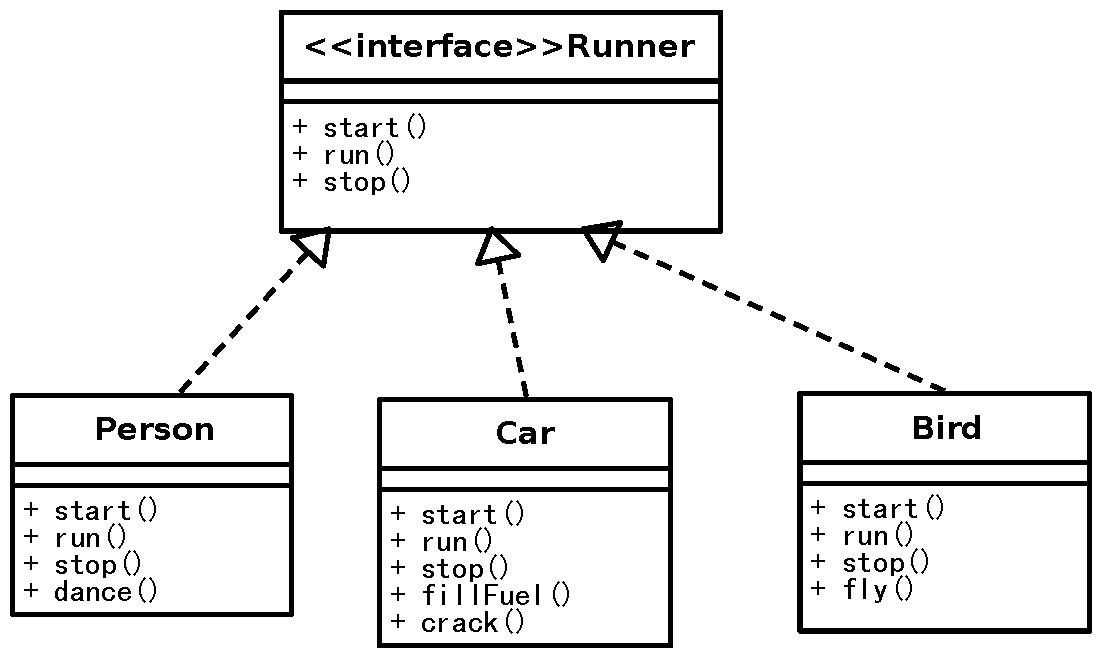
\includegraphics[width=0.6\textwidth]{images/Advanced-class-features/fig-interface-implement-sample.pdf}
\caption{接口实现示例}
\label{fig:interface-implement-sample}
\end{figure}

\notice{类允许实现多重接口}

\codeset{package sample.advance.interfacesample}

\subsection{接口间的继承}

与接口的多重实现情况类似,由于不担心方法追溯调用上的不确定性,接口之间
的继承允许“多重继承”的情况。

\begin{javaCode}
  interface A {
    public void ma();
  }
  interface B {
    public int mb(int i);
  }
  interface C extends A,B {  //接口的多重继承
    public String mc();
  }
  class D implements C {
    public void ma() {
      System.out.println("Implements method ma()!");
    }
    public int mb(int i) {
      return 2000 + i;
    }
    public String mc() {
      return "Hello!";
    }
  }
\end{javaCode}

上述代码中的D类缺省继承了Object类,直接实现了接口C,间接实现了接口A和B,
由于多态性的机制,将来D类的对象可以当作Object、C、A或B等类型使用。


\subsection{接口特性总结}

\begin{itemize}
\item 通过接口可以实现不相关类的相同行为,而不需要考虑这些类之间的层次关系。
\item 接口可以被多重实现。
\item 接口可以继承其它的接口,并添加新的属性和抽象方法,接口间支持多重继承。
\end{itemize}

\section{抽象类和接口剖析}

\subsection{语法层面的区别}

{\centering\hei\centering 概念差异 —— 语法差异 —— 用法差异 —— 设计哲学}

\begin{itemize}
\item 抽象类可以提供成员方法的实现细节,而接口中只能存在public
  abstract方法
\item 抽象类中的成员变量可以为各种类型,而接口中的成员变量只能
  是public static final类型
\item 抽象类可以有静态代码块和静态方法,接口中不能含有静态代码块以及
  静态方法
\item 一个类只能继承一个抽象类,而一个类却可以实现多个接口
\end{itemize}

\subsection{设计层面的区别}

\begin{itemize}
\item 抽象类是对类的抽象(可以抽象但不宜实例化),而接口是对行为的
  抽象。
\item 抽象类是对类整体进行抽象,包括属性、行为,但是接口却是对类局
  部(行为)进行抽象。
\end{itemize}


\begin{itemize}
\item 抽象类作为很多子类的父类,它是一种模板式设计。{\Red 模板式设计:模
    板代表公共部分,公共部分需要改的则改动模板即可。}
\item 而接口是一种行为规范,它是一种辐射式设计。{\Red 辐射式设计:接口
    进行了变更,则所有实现类都必须进行相应的改动。}
\end{itemize}



\subsection{怎样才是合理的设计?(门和警报的示例)}

以门和警报设计作为示例,一般来说,门都有\fbox{open()}和\fbox{close()}这
两个动作。通过抽象类和接口来定义这个抽象概念:

\begin{javaCode}
  abstract class Door {
    public abstract void open();
    public abstract void close();
  }
\end{javaCode}

\begin{javaCode}
  interface Door {
    public abstract void open();
    public abstract void close();
  }
\end{javaCode}

\notice{问题} 如果现在我们需要门具有报警\fbox{alarm()}的功能该如何实
现?

\subsubsection{思路一} 
  
将这三个功能都放在抽象类里面,这样一来所有继承这个抽象类的子类都具备
了报警功能,但是有的门并不一定需要具备报警功能。{\hei\Red 不合理抽象}

  
\subsubsection{思路二} 

将这三个功能都放在接口里面,但需要用到报警功能的类就需要实现这个接口
中的open()和close(),也许这个类根本就不具备open()和close()这两个功能,
比如火灾报警器。{\hei\Red 不合理规划}

Door的open() 、close()和alarm()根本就属于两个不同范畴内的行为:

\begin{itemize}
\item open()和close()属于门本身固有的行为特性。
\item alarm()属于延伸的附加行为。
\end{itemize}

\subsubsection{更为合理的思路} 

\ding{182} 单独将报警设计为一个接口,包含alarm()行为;\ding{183} Door设计为单独
的抽象类,包含open()和close()两种行为;\ding{184} 设计一个报警门继
承Door类和实现Alarm接口。

\codeset{package sample.advance.door}

\section{嵌套类}

\subsection{什么是嵌套类}

Java语言支持类的嵌套定义,即允许将一个类定义在其他类的内部,其中内层的类被称为嵌套类。

\subsubsection{嵌套类的分类}

\begin{description}
\item[\fbox{静态嵌套类(Static Nested Class)}] 使用static修饰的嵌套类
\item[\fbox{内部类(Inner Class)}] 非static的嵌套类
  \begin{description}
  \item[普通内部类] 在类中的方法或语句块外部定义的非static类。
  \item[局部内部类] 定义在方法或语句块中的类,也称局部类。
  \item[匿名内部类] 定义在方法或语句块中,该类没有名字、只能在其所在
    之处使用一次。
  \end{description}
\end{description}

\subsection{静态嵌套类}

\subsubsection{静态嵌套类的特征}

\begin{itemize}
\item {\hei 静态嵌套类不再依赖/引用外层类的特定对象,只是隐藏在另一个
    类中而已。}
\item 由于静态嵌套类的对象不依赖外层类的对象而独立存在,因而可以直接
  创建,进而也就无法在静态嵌套类中直接使用其外层类的非static成员。
\end{itemize}

\codeset{sample.advance.nestedclass.StaticNestedClassSample.java}

\subsection{匿名内部类}

匿名内部类是局部类的一种简化。

{\kai 当我们只在一处使用到某个类型时,可以将之定义为局部类,进而如果我
  们只是创建并使用该类的一个实例的话,那么连类的名字都可以省略。}

\subsection{使用匿名内部类}

\samp{Person.java}

\begin{javaCode}
  public abstract class Person {
    private String name;
    private int age;
    
    public Person() {}
    
    public Person(String name, int age) {
      this.name = name;
      this.age = age;
    }
    
    public String getInfo() {
      return "Name: " + name + "\t Age: " + age;
    }
    
    public abstract void work();
  }  
\end{javaCode}

\samp{TestAnonymous.java}

\begin{javaCode}
  public class TestAnonymous {
    public static void main(String[] args) {
      Person sp = new Person() { // 匿名内部类
        public void work() {
          System.out.println("个人信息:" + this.getInfo());
          System.out.println("I am sailing.");
        }
      };
      
      sp.work();
    }
  }
\end{javaCode}

对上述代码的解释如下:

{\kai 定义一个新的Java内部类,该类本身没有名字,但继承了指定的父类Person,并
在此匿名子类中重写了父类的work()方法,然后立即创建了一个该匿名子类的对
象,再将其地址保存到引用变量sp中待用。}


由于匿名类没有类名,而构造方法必须与类同名,所以{\hei 匿名类不能显式的
  定义构造方法},但系统允许在创建匿名类对象时将参数传给父类构造方法(使
用父类的构造方法)。

\begin{javaCode}
  Person sp = new Person("Kevin", 30) {
    public void work() {
      System.out.println("个人信息:" + this.getInfo());
      System.out.println("I am sailing.");
    }
  };
\end{javaCode}

匿名类除了可以继承现有父类之外,还可以实现接口,但不允许实现多个接口,
且实现接口时就不能再继承父类了,反之亦然。

\samp{Swimmer.java}

\begin{javaCode}
  public interface Swimmer {
    public abstract void swim();
  }
\end{javaCode}

\samp{TestAnonymous2.java}

\begin{javaCode}
  public class TestAnonymous2 {
    public static void main(String[] args) {
      TestAnonymous2 ta = new TestAnonymous2();
      ta.test(new Swimmer() { // 匿名类实现接口
        public void swim() {
          System.out.println("I am swimming.");
        }
      });
      
      public void test(Swimmer swimmer) {
        swimmer.swim();
      }
    }
  }
\end{javaCode}


\section{枚举类型}

\subsection{枚举类型的概念}

Java SE 5.0开始,引入了一种新的引用数据结构{\hei\Red 枚举类型}。{\kai
  枚举类型均自动继承java.lang.Enum类,使用一组常量值来表示特定的数据集
  合,该集合中数据的数目确定(通常较少),且这些数据只能取预先定义的值。}

\begin{javaCode}
  public enum Week {
    MON, TUE, WED, THU, FRI, SAT, SUN
  }
\end{javaCode}

\notice{无枚举类型前如何解决上述需求?}

一般采用声明多个整型常量的做法实现枚举类的功能。

\begin{javaCode}
  public class Week {
    public static final int MON = 1;
    public static final int TUE = 2;
    ...
  }    
\end{javaCode}


\subsection{遍历枚举类型常量值}

可以使用静态方法values()遍历枚举类型常量值。

\samp{ListEnum.java}

\begin{javaCode}
  public class ListEnum {
    public static void main(String[] args) {
      Week[] days = Week.values();
      for(Week d: days) {
        System.out.println(d);
      }
    }
  }
\end{javaCode}

\subsection{组合使用枚举类型与switch}

\codeset{package sample.advance.enumclass}

\notice{注意}

\begin{enumerate}
\item case字句必须省略其枚举类型的前缀,即只需要写成 case SUN:,而不允许写成 case
  Week.SUN:,否则编译出错。
\item 不必担心系统无法搞清这些常量名称的出处,因为switch后的小括号中的表达式已经指明本次
  要区分处理的是Week类型常量。
\end{enumerate}



\newpage
\section*{实验设计}
\sline